\documentclass[twoside]{book}

% Packages required by doxygen
\usepackage{fixltx2e}
\usepackage{calc}
\usepackage{doxygen}
\usepackage[export]{adjustbox} % also loads graphicx
\usepackage{graphicx}
\usepackage[utf8]{inputenc}
\usepackage{makeidx}
\usepackage{multicol}
\usepackage{multirow}
\PassOptionsToPackage{warn}{textcomp}
\usepackage{textcomp}
\usepackage[nointegrals]{wasysym}
\usepackage[table]{xcolor}

% Font selection
\usepackage[T1]{fontenc}
\usepackage[scaled=.90]{helvet}
\usepackage{courier}
\usepackage{amssymb}
\usepackage{sectsty}
\renewcommand{\familydefault}{\sfdefault}
\allsectionsfont{%
  \fontseries{bc}\selectfont%
  \color{darkgray}%
}
\renewcommand{\DoxyLabelFont}{%
  \fontseries{bc}\selectfont%
  \color{darkgray}%
}
\newcommand{\+}{\discretionary{\mbox{\scriptsize$\hookleftarrow$}}{}{}}

% Page & text layout
\usepackage{geometry}
\geometry{%
  a4paper,%
  top=2.5cm,%
  bottom=2.5cm,%
  left=2.5cm,%
  right=2.5cm%
}
\tolerance=750
\hfuzz=15pt
\hbadness=750
\setlength{\emergencystretch}{15pt}
\setlength{\parindent}{0cm}
\setlength{\parskip}{3ex plus 2ex minus 2ex}
\makeatletter
\renewcommand{\paragraph}{%
  \@startsection{paragraph}{4}{0ex}{-1.0ex}{1.0ex}{%
    \normalfont\normalsize\bfseries\SS@parafont%
  }%
}
\renewcommand{\subparagraph}{%
  \@startsection{subparagraph}{5}{0ex}{-1.0ex}{1.0ex}{%
    \normalfont\normalsize\bfseries\SS@subparafont%
  }%
}
\makeatother

% Headers & footers
\usepackage{fancyhdr}
\pagestyle{fancyplain}
\fancyhead[LE]{\fancyplain{}{\bfseries\thepage}}
\fancyhead[CE]{\fancyplain{}{}}
\fancyhead[RE]{\fancyplain{}{\bfseries\leftmark}}
\fancyhead[LO]{\fancyplain{}{\bfseries\rightmark}}
\fancyhead[CO]{\fancyplain{}{}}
\fancyhead[RO]{\fancyplain{}{\bfseries\thepage}}
\fancyfoot[LE]{\fancyplain{}{}}
\fancyfoot[CE]{\fancyplain{}{}}
\fancyfoot[RE]{\fancyplain{}{\bfseries\scriptsize Generated by Doxygen }}
\fancyfoot[LO]{\fancyplain{}{\bfseries\scriptsize Generated by Doxygen }}
\fancyfoot[CO]{\fancyplain{}{}}
\fancyfoot[RO]{\fancyplain{}{}}
\renewcommand{\footrulewidth}{0.4pt}
\renewcommand{\chaptermark}[1]{%
  \markboth{#1}{}%
}
\renewcommand{\sectionmark}[1]{%
  \markright{\thesection\ #1}%
}

% Indices & bibliography
\usepackage{natbib}
\usepackage[titles]{tocloft}
\setcounter{tocdepth}{3}
\setcounter{secnumdepth}{5}
\makeindex

% Hyperlinks (required, but should be loaded last)
\usepackage{ifpdf}
\ifpdf
  \usepackage[pdftex,pagebackref=true]{hyperref}
\else
  \usepackage[ps2pdf,pagebackref=true]{hyperref}
\fi
\hypersetup{%
  colorlinks=true,%
  linkcolor=blue,%
  citecolor=blue,%
  unicode%
}

% Custom commands
\newcommand{\clearemptydoublepage}{%
  \newpage{\pagestyle{empty}\cleardoublepage}%
}

\usepackage{caption}
\captionsetup{labelsep=space,justification=centering,font={bf},singlelinecheck=off,skip=4pt,position=top}

%===== C O N T E N T S =====

\begin{document}

% Titlepage & ToC
\hypersetup{pageanchor=false,
             bookmarksnumbered=true,
             pdfencoding=unicode
            }
\pagenumbering{alph}
\begin{titlepage}
\vspace*{7cm}
\begin{center}%
{\Large 809Y Final Project (Novak, Pittman, Smith) \\[1ex]\large 1.\+0 }\\
\vspace*{1cm}
{\large Generated by Doxygen 1.8.13}\\
\end{center}
\end{titlepage}
\clearemptydoublepage
\pagenumbering{roman}
\tableofcontents
\clearemptydoublepage
\pagenumbering{arabic}
\hypersetup{pageanchor=true}

%--- Begin generated contents ---
\chapter{final\+\_\+project}
\label{md__r_e_a_d_m_e}
\Hypertarget{md__r_e_a_d_m_e}
Non-\/complete package for the final project for\+: E\+N\+P\+M809Y Fall 2021


\begin{DoxyItemize}
\item The {\ttfamily doc} folder contains the instructions.
\item The {\ttfamily script} folder contains install.\+bash to install required packages. 
\end{DoxyItemize}
\chapter{Class Index}
\section{Class List}
Here are the classes, structs, unions and interfaces with brief descriptions\+:\begin{DoxyCompactList}
\item\contentsline{section}{\hyperlink{class_bot___controller}{Bot\+\_\+\+Controller} \\*Controller class to drive a turtlebot }{\pageref{class_bot___controller}}{}
\item\contentsline{section}{\hyperlink{class_explorer}{Explorer} \\*A class that inherits from Bot\+\_\+contreoller to control the explorer and exploration algorithm }{\pageref{class_explorer}}{}
\item\contentsline{section}{\hyperlink{class_follower}{Follower} \\*\hyperlink{class_follower}{Follower} Class \hyperlink{class_explorer}{Explorer} }{\pageref{class_follower}}{}
\end{DoxyCompactList}

\chapter{File Index}
\section{File List}
Here is a list of all files with brief descriptions\+:\begin{DoxyCompactList}
\item\contentsline{section}{include/explorer/\hyperlink{aruco__confirm_8h}{aruco\+\_\+confirm.\+h} }{\pageref{aruco__confirm_8h}}{}
\item\contentsline{section}{include/explorer/\hyperlink{explorer_8h}{explorer.\+h} }{\pageref{explorer_8h}}{}
\item\contentsline{section}{include/follower/\hyperlink{follower_8h}{follower.\+h} }{\pageref{follower_8h}}{}
\item\contentsline{section}{src/\hyperlink{aruco__confirm_8cpp}{aruco\+\_\+confirm.\+cpp} }{\pageref{aruco__confirm_8cpp}}{}
\item\contentsline{section}{src/\hyperlink{explorer_8cpp}{explorer.\+cpp} \\*\hyperlink{class_aruco_node}{Aruco\+Node} }{\pageref{explorer_8cpp}}{}
\item\contentsline{section}{src/\hyperlink{follower_8cpp}{follower.\+cpp} \\*\hyperlink{class_follower}{Follower} Robot }{\pageref{follower_8cpp}}{}
\item\contentsline{section}{src/\hyperlink{main_8cpp}{main.\+cpp} \\*809Y Final Project Group 5 }{\pageref{main_8cpp}}{}
\end{DoxyCompactList}

\chapter{Class Documentation}
\hypertarget{class_bot___controller}{}\section{Bot\+\_\+\+Controller Class Reference}
\label{class_bot___controller}\index{Bot\+\_\+\+Controller@{Bot\+\_\+\+Controller}}


Controller class to drive a turtlebot.  




{\ttfamily \#include $<$bot\+\_\+controller.\+h$>$}

\subsection*{Public Member Functions}
\begin{DoxyCompactItemize}
\item 
\hyperlink{class_bot___controller_a05104e1b41f7c9cd9cdfe80bbbd53a7d}{Bot\+\_\+\+Controller} (ros\+::\+Node\+Handle $\ast$nodehandle, const std\+::string \&robot\+\_\+name)
\item 
void \hyperlink{class_bot___controller_a7c4af8b19d122f72582b5bbd309ded7a}{publish\+\_\+velocities} (const geometry\+\_\+msgs\+::\+Twist \&msg)
\item 
void \hyperlink{class_bot___controller_aacde4d9a862dfa0fc029686a66603de7}{drive\+\_\+straight} (double distance, bool direction)
\item 
void \hyperlink{class_bot___controller_a8ea05eaf643a647581a0f60ab9c85c24}{rotate} (double angle\+\_\+to\+\_\+rotate, bool direction, double final\+\_\+angle)
\item 
bool \hyperlink{class_bot___controller_a7bd188779f02159f9fdfea435caf94b1}{go\+\_\+to\+\_\+goal} (double x, double y)
\item 
void \hyperlink{class_bot___controller_a87e3ac792f943a573e676d382a816519}{stop} ()
\item 
double \hyperlink{class_bot___controller_a25e004b632ad2c2c494f8a91f3c24533}{compute\+\_\+expected\+\_\+final\+\_\+yaw} (bool direction, double angle\+\_\+to\+\_\+rotate)
\item 
double \hyperlink{class_bot___controller_ad9ed858063dc3f928157122e95e677ae}{compute\+\_\+yaw\+\_\+deg} ()
\item 
double \hyperlink{class_bot___controller_af23e3dd2a3af58bc16fda4aebbd78c18}{compute\+\_\+yaw\+\_\+rad} ()
\item 
double \hyperlink{class_bot___controller_ad07d6cfa7f66b200a1540221b699b48e}{convert\+\_\+rad\+\_\+to\+\_\+deg} (double angle)
\item 
const double \hyperlink{class_bot___controller_a2efd33efbb2d3c8caa52e04a049b5971}{get\+\_\+current\+\_\+x} ()
\item 
const double \hyperlink{class_bot___controller_a5985b03ff6787846a5abf5cd85ed6ae2}{get\+\_\+current\+\_\+y} ()
\end{DoxyCompactItemize}


\subsection{Detailed Description}
Controller class to drive a turtlebot. 

Definition at line 16 of file bot\+\_\+controller.\+h.



\subsection{Constructor \& Destructor Documentation}
\mbox{\Hypertarget{class_bot___controller_a05104e1b41f7c9cd9cdfe80bbbd53a7d}\label{class_bot___controller_a05104e1b41f7c9cd9cdfe80bbbd53a7d}} 
\index{Bot\+\_\+\+Controller@{Bot\+\_\+\+Controller}!Bot\+\_\+\+Controller@{Bot\+\_\+\+Controller}}
\index{Bot\+\_\+\+Controller@{Bot\+\_\+\+Controller}!Bot\+\_\+\+Controller@{Bot\+\_\+\+Controller}}
\subsubsection{\texorpdfstring{Bot\+\_\+\+Controller()}{Bot\_Controller()}}
{\footnotesize\ttfamily Bot\+\_\+\+Controller\+::\+Bot\+\_\+\+Controller (\begin{DoxyParamCaption}\item[{ros\+::\+Node\+Handle $\ast$}]{nodehandle,  }\item[{const std\+::string \&}]{robot\+\_\+name }\end{DoxyParamCaption})}



Definition at line 8 of file bot\+\_\+controller.\+cpp.



\subsection{Member Function Documentation}
\mbox{\Hypertarget{class_bot___controller_a25e004b632ad2c2c494f8a91f3c24533}\label{class_bot___controller_a25e004b632ad2c2c494f8a91f3c24533}} 
\index{Bot\+\_\+\+Controller@{Bot\+\_\+\+Controller}!compute\+\_\+expected\+\_\+final\+\_\+yaw@{compute\+\_\+expected\+\_\+final\+\_\+yaw}}
\index{compute\+\_\+expected\+\_\+final\+\_\+yaw@{compute\+\_\+expected\+\_\+final\+\_\+yaw}!Bot\+\_\+\+Controller@{Bot\+\_\+\+Controller}}
\subsubsection{\texorpdfstring{compute\+\_\+expected\+\_\+final\+\_\+yaw()}{compute\_expected\_final\_yaw()}}
{\footnotesize\ttfamily double Bot\+\_\+\+Controller\+::compute\+\_\+expected\+\_\+final\+\_\+yaw (\begin{DoxyParamCaption}\item[{bool}]{direction,  }\item[{double}]{angle\+\_\+to\+\_\+rotate }\end{DoxyParamCaption})}



Definition at line 95 of file bot\+\_\+controller.\+cpp.

\mbox{\Hypertarget{class_bot___controller_ad9ed858063dc3f928157122e95e677ae}\label{class_bot___controller_ad9ed858063dc3f928157122e95e677ae}} 
\index{Bot\+\_\+\+Controller@{Bot\+\_\+\+Controller}!compute\+\_\+yaw\+\_\+deg@{compute\+\_\+yaw\+\_\+deg}}
\index{compute\+\_\+yaw\+\_\+deg@{compute\+\_\+yaw\+\_\+deg}!Bot\+\_\+\+Controller@{Bot\+\_\+\+Controller}}
\subsubsection{\texorpdfstring{compute\+\_\+yaw\+\_\+deg()}{compute\_yaw\_deg()}}
{\footnotesize\ttfamily double Bot\+\_\+\+Controller\+::compute\+\_\+yaw\+\_\+deg (\begin{DoxyParamCaption}{ }\end{DoxyParamCaption})}



Definition at line 110 of file bot\+\_\+controller.\+cpp.

\mbox{\Hypertarget{class_bot___controller_af23e3dd2a3af58bc16fda4aebbd78c18}\label{class_bot___controller_af23e3dd2a3af58bc16fda4aebbd78c18}} 
\index{Bot\+\_\+\+Controller@{Bot\+\_\+\+Controller}!compute\+\_\+yaw\+\_\+rad@{compute\+\_\+yaw\+\_\+rad}}
\index{compute\+\_\+yaw\+\_\+rad@{compute\+\_\+yaw\+\_\+rad}!Bot\+\_\+\+Controller@{Bot\+\_\+\+Controller}}
\subsubsection{\texorpdfstring{compute\+\_\+yaw\+\_\+rad()}{compute\_yaw\_rad()}}
{\footnotesize\ttfamily double Bot\+\_\+\+Controller\+::compute\+\_\+yaw\+\_\+rad (\begin{DoxyParamCaption}{ }\end{DoxyParamCaption})}



Definition at line 128 of file bot\+\_\+controller.\+cpp.

\mbox{\Hypertarget{class_bot___controller_ad07d6cfa7f66b200a1540221b699b48e}\label{class_bot___controller_ad07d6cfa7f66b200a1540221b699b48e}} 
\index{Bot\+\_\+\+Controller@{Bot\+\_\+\+Controller}!convert\+\_\+rad\+\_\+to\+\_\+deg@{convert\+\_\+rad\+\_\+to\+\_\+deg}}
\index{convert\+\_\+rad\+\_\+to\+\_\+deg@{convert\+\_\+rad\+\_\+to\+\_\+deg}!Bot\+\_\+\+Controller@{Bot\+\_\+\+Controller}}
\subsubsection{\texorpdfstring{convert\+\_\+rad\+\_\+to\+\_\+deg()}{convert\_rad\_to\_deg()}}
{\footnotesize\ttfamily double Bot\+\_\+\+Controller\+::convert\+\_\+rad\+\_\+to\+\_\+deg (\begin{DoxyParamCaption}\item[{double}]{angle }\end{DoxyParamCaption})}



Definition at line 56 of file bot\+\_\+controller.\+cpp.

\mbox{\Hypertarget{class_bot___controller_aacde4d9a862dfa0fc029686a66603de7}\label{class_bot___controller_aacde4d9a862dfa0fc029686a66603de7}} 
\index{Bot\+\_\+\+Controller@{Bot\+\_\+\+Controller}!drive\+\_\+straight@{drive\+\_\+straight}}
\index{drive\+\_\+straight@{drive\+\_\+straight}!Bot\+\_\+\+Controller@{Bot\+\_\+\+Controller}}
\subsubsection{\texorpdfstring{drive\+\_\+straight()}{drive\_straight()}}
{\footnotesize\ttfamily void Bot\+\_\+\+Controller\+::drive\+\_\+straight (\begin{DoxyParamCaption}\item[{double}]{distance,  }\item[{bool}]{direction }\end{DoxyParamCaption})}



Definition at line 173 of file bot\+\_\+controller.\+cpp.

\mbox{\Hypertarget{class_bot___controller_a2efd33efbb2d3c8caa52e04a049b5971}\label{class_bot___controller_a2efd33efbb2d3c8caa52e04a049b5971}} 
\index{Bot\+\_\+\+Controller@{Bot\+\_\+\+Controller}!get\+\_\+current\+\_\+x@{get\+\_\+current\+\_\+x}}
\index{get\+\_\+current\+\_\+x@{get\+\_\+current\+\_\+x}!Bot\+\_\+\+Controller@{Bot\+\_\+\+Controller}}
\subsubsection{\texorpdfstring{get\+\_\+current\+\_\+x()}{get\_current\_x()}}
{\footnotesize\ttfamily const double Bot\+\_\+\+Controller\+::get\+\_\+current\+\_\+x (\begin{DoxyParamCaption}{ }\end{DoxyParamCaption})\hspace{0.3cm}{\ttfamily [inline]}}



Definition at line 31 of file bot\+\_\+controller.\+h.

\mbox{\Hypertarget{class_bot___controller_a5985b03ff6787846a5abf5cd85ed6ae2}\label{class_bot___controller_a5985b03ff6787846a5abf5cd85ed6ae2}} 
\index{Bot\+\_\+\+Controller@{Bot\+\_\+\+Controller}!get\+\_\+current\+\_\+y@{get\+\_\+current\+\_\+y}}
\index{get\+\_\+current\+\_\+y@{get\+\_\+current\+\_\+y}!Bot\+\_\+\+Controller@{Bot\+\_\+\+Controller}}
\subsubsection{\texorpdfstring{get\+\_\+current\+\_\+y()}{get\_current\_y()}}
{\footnotesize\ttfamily const double Bot\+\_\+\+Controller\+::get\+\_\+current\+\_\+y (\begin{DoxyParamCaption}{ }\end{DoxyParamCaption})\hspace{0.3cm}{\ttfamily [inline]}}



Definition at line 35 of file bot\+\_\+controller.\+h.

\mbox{\Hypertarget{class_bot___controller_a7bd188779f02159f9fdfea435caf94b1}\label{class_bot___controller_a7bd188779f02159f9fdfea435caf94b1}} 
\index{Bot\+\_\+\+Controller@{Bot\+\_\+\+Controller}!go\+\_\+to\+\_\+goal@{go\+\_\+to\+\_\+goal}}
\index{go\+\_\+to\+\_\+goal@{go\+\_\+to\+\_\+goal}!Bot\+\_\+\+Controller@{Bot\+\_\+\+Controller}}
\subsubsection{\texorpdfstring{go\+\_\+to\+\_\+goal()}{go\_to\_goal()}}
{\footnotesize\ttfamily bool Bot\+\_\+\+Controller\+::go\+\_\+to\+\_\+goal (\begin{DoxyParamCaption}\item[{double}]{x,  }\item[{double}]{y }\end{DoxyParamCaption})}



Definition at line 195 of file bot\+\_\+controller.\+cpp.

\mbox{\Hypertarget{class_bot___controller_a7c4af8b19d122f72582b5bbd309ded7a}\label{class_bot___controller_a7c4af8b19d122f72582b5bbd309ded7a}} 
\index{Bot\+\_\+\+Controller@{Bot\+\_\+\+Controller}!publish\+\_\+velocities@{publish\+\_\+velocities}}
\index{publish\+\_\+velocities@{publish\+\_\+velocities}!Bot\+\_\+\+Controller@{Bot\+\_\+\+Controller}}
\subsubsection{\texorpdfstring{publish\+\_\+velocities()}{publish\_velocities()}}
{\footnotesize\ttfamily void Bot\+\_\+\+Controller\+::publish\+\_\+velocities (\begin{DoxyParamCaption}\item[{const geometry\+\_\+msgs\+::\+Twist \&}]{msg }\end{DoxyParamCaption})}

\mbox{\Hypertarget{class_bot___controller_a8ea05eaf643a647581a0f60ab9c85c24}\label{class_bot___controller_a8ea05eaf643a647581a0f60ab9c85c24}} 
\index{Bot\+\_\+\+Controller@{Bot\+\_\+\+Controller}!rotate@{rotate}}
\index{rotate@{rotate}!Bot\+\_\+\+Controller@{Bot\+\_\+\+Controller}}
\subsubsection{\texorpdfstring{rotate()}{rotate()}}
{\footnotesize\ttfamily void Bot\+\_\+\+Controller\+::rotate (\begin{DoxyParamCaption}\item[{double}]{angle\+\_\+to\+\_\+rotate,  }\item[{bool}]{direction,  }\item[{double}]{final\+\_\+angle }\end{DoxyParamCaption})}



Definition at line 146 of file bot\+\_\+controller.\+cpp.

\mbox{\Hypertarget{class_bot___controller_a87e3ac792f943a573e676d382a816519}\label{class_bot___controller_a87e3ac792f943a573e676d382a816519}} 
\index{Bot\+\_\+\+Controller@{Bot\+\_\+\+Controller}!stop@{stop}}
\index{stop@{stop}!Bot\+\_\+\+Controller@{Bot\+\_\+\+Controller}}
\subsubsection{\texorpdfstring{stop()}{stop()}}
{\footnotesize\ttfamily void Bot\+\_\+\+Controller\+::stop (\begin{DoxyParamCaption}{ }\end{DoxyParamCaption})}



Definition at line 86 of file bot\+\_\+controller.\+cpp.



The documentation for this class was generated from the following files\+:\begin{DoxyCompactItemize}
\item 
include/\hyperlink{bot__controller_8h}{bot\+\_\+controller.\+h}\item 
src/\hyperlink{bot__controller_8cpp}{bot\+\_\+controller.\+cpp}\end{DoxyCompactItemize}

\hypertarget{class_explorer}{}\section{Explorer Class Reference}
\label{class_explorer}\index{Explorer@{Explorer}}


A class that inherits from Bot\+\_\+contreoller to control the explorer and exploration algorithm.  




{\ttfamily \#include $<$explorer.\+h$>$}

\subsection*{Public Member Functions}
\begin{DoxyCompactItemize}
\item 
\hyperlink{class_explorer_aafe6b7c3b9c2e24815aa14a731f31890}{Explorer} (ros\+::\+Node\+Handle $\ast$nodehandle, const std\+::string \&robot\+\_\+name)
\item 
void \hyperlink{class_explorer_a8ffef25585ef957b9df4407366723787}{publish\+\_\+velocities} (const geometry\+\_\+msgs\+::\+Twist \&msg)
\item 
void \hyperlink{class_explorer_ab4ca9f16c48a60fc4d0e426b6fd9e9a0}{drive\+\_\+straight} (double distance, bool direction)
\item 
void \hyperlink{class_explorer_ac8e3a980fd3929734fb3a4b0b2e0a7e0}{rotate} (double angle\+\_\+to\+\_\+rotate, bool direction, double final\+\_\+angle)
\item 
bool \hyperlink{class_explorer_aa1e259feaac1114adb0f24588428e8ef}{go\+\_\+to\+\_\+goal} (double x, double y)
\item 
void \hyperlink{class_explorer_a0e4a623ff30d1886cc9f57ec081c527f}{stop} ()
\item 
double \hyperlink{class_explorer_a02c37b93448ed474f1bf0d03e2758ca2}{compute\+\_\+expected\+\_\+final\+\_\+yaw} (bool direction, double angle\+\_\+to\+\_\+rotate)
\item 
double \hyperlink{class_explorer_a670cdffdb8c3173c300590cfc45ab6d2}{compute\+\_\+yaw\+\_\+deg} ()
\item 
double \hyperlink{class_explorer_ac5b91cd64189a60ffe62535cb5bc093a}{compute\+\_\+yaw\+\_\+rad} ()
\item 
double \hyperlink{class_explorer_ac3a5c9368647dd9d2c36d12497bd889e}{convert\+\_\+rad\+\_\+to\+\_\+deg} (double angle)
\item 
\hyperlink{class_explorer_aa1b0a71e92e003e9162a5ba99d843392}{$\sim$\+Explorer} ()
\item 
void \hyperlink{class_explorer_a2b0c1e46e1a17e99f4156edf5a93b691}{move\+\_\+next\+\_\+loc} (std\+::array$<$ double, 2 $>$ goal\+\_\+loc)
\item 
std\+::array$<$ std\+::array$<$ double, 2 $>$, 4 $>$ \hyperlink{class_explorer_a847e3ad2e7233d493a8dcfdd7139cb58}{get\+\_\+goals} ()
\end{DoxyCompactItemize}
\subsection*{Public Attributes}
\begin{DoxyCompactItemize}
\item 
std\+::array$<$ std\+::array$<$ int, 3 $>$, 4 $>$ \hyperlink{class_explorer_acda1856f421dfe836f39de446415b969}{goal\+\_\+list} \{\}
\item 
std\+::array$<$ int, 3 $>$ \hyperlink{class_explorer_af1aee46522a58db39d3643f2138c76fa}{start\+\_\+place} \{\}
\end{DoxyCompactItemize}


\subsection{Detailed Description}
A class that inherits from Bot\+\_\+contreoller to control the explorer and exploration algorithm. 

Definition at line 10 of file explorer.\+h.



\subsection{Constructor \& Destructor Documentation}
\mbox{\Hypertarget{class_explorer_aafe6b7c3b9c2e24815aa14a731f31890}\label{class_explorer_aafe6b7c3b9c2e24815aa14a731f31890}} 
\index{Explorer@{Explorer}!Explorer@{Explorer}}
\index{Explorer@{Explorer}!Explorer@{Explorer}}
\subsubsection{\texorpdfstring{Explorer()}{Explorer()}}
{\footnotesize\ttfamily Explorer\+::\+Explorer (\begin{DoxyParamCaption}\item[{ros\+::\+Node\+Handle $\ast$}]{nodehandle,  }\item[{const std\+::string \&}]{robot\+\_\+name }\end{DoxyParamCaption})}



Definition at line 13 of file explorer.\+cpp.

\mbox{\Hypertarget{class_explorer_aa1b0a71e92e003e9162a5ba99d843392}\label{class_explorer_aa1b0a71e92e003e9162a5ba99d843392}} 
\index{Explorer@{Explorer}!````~Explorer@{$\sim$\+Explorer}}
\index{````~Explorer@{$\sim$\+Explorer}!Explorer@{Explorer}}
\subsubsection{\texorpdfstring{$\sim$\+Explorer()}{~Explorer()}}
{\footnotesize\ttfamily Explorer\+::$\sim$\+Explorer (\begin{DoxyParamCaption}{ }\end{DoxyParamCaption})\hspace{0.3cm}{\ttfamily [inline]}}



Definition at line 24 of file explorer.\+h.



\subsection{Member Function Documentation}
\mbox{\Hypertarget{class_explorer_a02c37b93448ed474f1bf0d03e2758ca2}\label{class_explorer_a02c37b93448ed474f1bf0d03e2758ca2}} 
\index{Explorer@{Explorer}!compute\+\_\+expected\+\_\+final\+\_\+yaw@{compute\+\_\+expected\+\_\+final\+\_\+yaw}}
\index{compute\+\_\+expected\+\_\+final\+\_\+yaw@{compute\+\_\+expected\+\_\+final\+\_\+yaw}!Explorer@{Explorer}}
\subsubsection{\texorpdfstring{compute\+\_\+expected\+\_\+final\+\_\+yaw()}{compute\_expected\_final\_yaw()}}
{\footnotesize\ttfamily double Explorer\+::compute\+\_\+expected\+\_\+final\+\_\+yaw (\begin{DoxyParamCaption}\item[{bool}]{direction,  }\item[{double}]{angle\+\_\+to\+\_\+rotate }\end{DoxyParamCaption})}



Definition at line 132 of file explorer.\+cpp.

\mbox{\Hypertarget{class_explorer_a670cdffdb8c3173c300590cfc45ab6d2}\label{class_explorer_a670cdffdb8c3173c300590cfc45ab6d2}} 
\index{Explorer@{Explorer}!compute\+\_\+yaw\+\_\+deg@{compute\+\_\+yaw\+\_\+deg}}
\index{compute\+\_\+yaw\+\_\+deg@{compute\+\_\+yaw\+\_\+deg}!Explorer@{Explorer}}
\subsubsection{\texorpdfstring{compute\+\_\+yaw\+\_\+deg()}{compute\_yaw\_deg()}}
{\footnotesize\ttfamily double Explorer\+::compute\+\_\+yaw\+\_\+deg (\begin{DoxyParamCaption}{ }\end{DoxyParamCaption})}



Definition at line 144 of file explorer.\+cpp.

\mbox{\Hypertarget{class_explorer_ac5b91cd64189a60ffe62535cb5bc093a}\label{class_explorer_ac5b91cd64189a60ffe62535cb5bc093a}} 
\index{Explorer@{Explorer}!compute\+\_\+yaw\+\_\+rad@{compute\+\_\+yaw\+\_\+rad}}
\index{compute\+\_\+yaw\+\_\+rad@{compute\+\_\+yaw\+\_\+rad}!Explorer@{Explorer}}
\subsubsection{\texorpdfstring{compute\+\_\+yaw\+\_\+rad()}{compute\_yaw\_rad()}}
{\footnotesize\ttfamily double Explorer\+::compute\+\_\+yaw\+\_\+rad (\begin{DoxyParamCaption}{ }\end{DoxyParamCaption})}



Definition at line 156 of file explorer.\+cpp.

\mbox{\Hypertarget{class_explorer_ac3a5c9368647dd9d2c36d12497bd889e}\label{class_explorer_ac3a5c9368647dd9d2c36d12497bd889e}} 
\index{Explorer@{Explorer}!convert\+\_\+rad\+\_\+to\+\_\+deg@{convert\+\_\+rad\+\_\+to\+\_\+deg}}
\index{convert\+\_\+rad\+\_\+to\+\_\+deg@{convert\+\_\+rad\+\_\+to\+\_\+deg}!Explorer@{Explorer}}
\subsubsection{\texorpdfstring{convert\+\_\+rad\+\_\+to\+\_\+deg()}{convert\_rad\_to\_deg()}}
{\footnotesize\ttfamily double Explorer\+::convert\+\_\+rad\+\_\+to\+\_\+deg (\begin{DoxyParamCaption}\item[{double}]{angle }\end{DoxyParamCaption})}



Definition at line 58 of file explorer.\+cpp.

\mbox{\Hypertarget{class_explorer_ab4ca9f16c48a60fc4d0e426b6fd9e9a0}\label{class_explorer_ab4ca9f16c48a60fc4d0e426b6fd9e9a0}} 
\index{Explorer@{Explorer}!drive\+\_\+straight@{drive\+\_\+straight}}
\index{drive\+\_\+straight@{drive\+\_\+straight}!Explorer@{Explorer}}
\subsubsection{\texorpdfstring{drive\+\_\+straight()}{drive\_straight()}}
{\footnotesize\ttfamily void Explorer\+::drive\+\_\+straight (\begin{DoxyParamCaption}\item[{double}]{distance,  }\item[{bool}]{direction }\end{DoxyParamCaption})}



Definition at line 195 of file explorer.\+cpp.

\mbox{\Hypertarget{class_explorer_a847e3ad2e7233d493a8dcfdd7139cb58}\label{class_explorer_a847e3ad2e7233d493a8dcfdd7139cb58}} 
\index{Explorer@{Explorer}!get\+\_\+goals@{get\+\_\+goals}}
\index{get\+\_\+goals@{get\+\_\+goals}!Explorer@{Explorer}}
\subsubsection{\texorpdfstring{get\+\_\+goals()}{get\_goals()}}
{\footnotesize\ttfamily std\+::array$<$std\+::array$<$double,2$>$,4$>$ Explorer\+::get\+\_\+goals (\begin{DoxyParamCaption}{ }\end{DoxyParamCaption})\hspace{0.3cm}{\ttfamily [inline]}}



Definition at line 33 of file explorer.\+h.

\mbox{\Hypertarget{class_explorer_aa1e259feaac1114adb0f24588428e8ef}\label{class_explorer_aa1e259feaac1114adb0f24588428e8ef}} 
\index{Explorer@{Explorer}!go\+\_\+to\+\_\+goal@{go\+\_\+to\+\_\+goal}}
\index{go\+\_\+to\+\_\+goal@{go\+\_\+to\+\_\+goal}!Explorer@{Explorer}}
\subsubsection{\texorpdfstring{go\+\_\+to\+\_\+goal()}{go\_to\_goal()}}
{\footnotesize\ttfamily bool Explorer\+::go\+\_\+to\+\_\+goal (\begin{DoxyParamCaption}\item[{double}]{x,  }\item[{double}]{y }\end{DoxyParamCaption})}



Definition at line 216 of file explorer.\+cpp.

\mbox{\Hypertarget{class_explorer_a2b0c1e46e1a17e99f4156edf5a93b691}\label{class_explorer_a2b0c1e46e1a17e99f4156edf5a93b691}} 
\index{Explorer@{Explorer}!move\+\_\+next\+\_\+loc@{move\+\_\+next\+\_\+loc}}
\index{move\+\_\+next\+\_\+loc@{move\+\_\+next\+\_\+loc}!Explorer@{Explorer}}
\subsubsection{\texorpdfstring{move\+\_\+next\+\_\+loc()}{move\_next\_loc()}}
{\footnotesize\ttfamily void Explorer\+::move\+\_\+next\+\_\+loc (\begin{DoxyParamCaption}\item[{std\+::array$<$ double, 2 $>$}]{goal\+\_\+loc }\end{DoxyParamCaption})\hspace{0.3cm}{\ttfamily [inline]}}



Definition at line 31 of file explorer.\+h.

\mbox{\Hypertarget{class_explorer_a8ffef25585ef957b9df4407366723787}\label{class_explorer_a8ffef25585ef957b9df4407366723787}} 
\index{Explorer@{Explorer}!publish\+\_\+velocities@{publish\+\_\+velocities}}
\index{publish\+\_\+velocities@{publish\+\_\+velocities}!Explorer@{Explorer}}
\subsubsection{\texorpdfstring{publish\+\_\+velocities()}{publish\_velocities()}}
{\footnotesize\ttfamily void Explorer\+::publish\+\_\+velocities (\begin{DoxyParamCaption}\item[{const geometry\+\_\+msgs\+::\+Twist \&}]{msg }\end{DoxyParamCaption})}

\mbox{\Hypertarget{class_explorer_ac8e3a980fd3929734fb3a4b0b2e0a7e0}\label{class_explorer_ac8e3a980fd3929734fb3a4b0b2e0a7e0}} 
\index{Explorer@{Explorer}!rotate@{rotate}}
\index{rotate@{rotate}!Explorer@{Explorer}}
\subsubsection{\texorpdfstring{rotate()}{rotate()}}
{\footnotesize\ttfamily void Explorer\+::rotate (\begin{DoxyParamCaption}\item[{double}]{angle\+\_\+to\+\_\+rotate,  }\item[{bool}]{direction,  }\item[{double}]{final\+\_\+angle }\end{DoxyParamCaption})}



Definition at line 168 of file explorer.\+cpp.

\mbox{\Hypertarget{class_explorer_a0e4a623ff30d1886cc9f57ec081c527f}\label{class_explorer_a0e4a623ff30d1886cc9f57ec081c527f}} 
\index{Explorer@{Explorer}!stop@{stop}}
\index{stop@{stop}!Explorer@{Explorer}}
\subsubsection{\texorpdfstring{stop()}{stop()}}
{\footnotesize\ttfamily void Explorer\+::stop (\begin{DoxyParamCaption}{ }\end{DoxyParamCaption})}



Definition at line 123 of file explorer.\+cpp.



\subsection{Member Data Documentation}
\mbox{\Hypertarget{class_explorer_acda1856f421dfe836f39de446415b969}\label{class_explorer_acda1856f421dfe836f39de446415b969}} 
\index{Explorer@{Explorer}!goal\+\_\+list@{goal\+\_\+list}}
\index{goal\+\_\+list@{goal\+\_\+list}!Explorer@{Explorer}}
\subsubsection{\texorpdfstring{goal\+\_\+list}{goal\_list}}
{\footnotesize\ttfamily std\+::array$<$std\+::array$<$int,3$>$,4$>$ Explorer\+::goal\+\_\+list \{\}}



Definition at line 27 of file explorer.\+h.

\mbox{\Hypertarget{class_explorer_af1aee46522a58db39d3643f2138c76fa}\label{class_explorer_af1aee46522a58db39d3643f2138c76fa}} 
\index{Explorer@{Explorer}!start\+\_\+place@{start\+\_\+place}}
\index{start\+\_\+place@{start\+\_\+place}!Explorer@{Explorer}}
\subsubsection{\texorpdfstring{start\+\_\+place}{start\_place}}
{\footnotesize\ttfamily std\+::array$<$int,3$>$ Explorer\+::start\+\_\+place \{\}}



Definition at line 28 of file explorer.\+h.



The documentation for this class was generated from the following files\+:\begin{DoxyCompactItemize}
\item 
include/explorer/\hyperlink{explorer_8h}{explorer.\+h}\item 
src/\hyperlink{explorer_8cpp}{explorer.\+cpp}\end{DoxyCompactItemize}

\hypertarget{class_follower}{}\section{Follower Class Reference}
\label{class_follower}\index{Follower@{Follower}}


\hyperlink{class_follower}{Follower} Class for \hyperlink{class_follower}{Follower} bot Goal is to have \hyperlink{class_follower}{Follower} go to Ar\+Uco markers in fiducial ID order.  




{\ttfamily \#include $<$follower.\+h$>$}

\subsection*{Public Member Functions}
\begin{DoxyCompactItemize}
\item 
\hyperlink{class_follower_a6870e654b7cc901944ead12870a6b107}{Follower} (ros\+::\+Node\+Handle $\ast$nodehandle, const std\+::string \&robot\+\_\+name)
\begin{DoxyCompactList}\small\item\em Construct a new \hyperlink{class_follower}{Follower} object. \end{DoxyCompactList}\item 
void \hyperlink{class_follower_aaae1600959a929c269d557d9c09ba777}{publish\+\_\+velocities} (const geometry\+\_\+msgs\+::\+Twist \&msg)
\begin{DoxyCompactList}\small\item\em Publish velocities to odom. \end{DoxyCompactList}\item 
void \hyperlink{class_follower_ad4d1ce6f43ce65c0aa5a560247ca55ad}{drive\+\_\+straight} (double distance, bool direction)
\begin{DoxyCompactList}\small\item\em moves robot straight \end{DoxyCompactList}\item 
void \hyperlink{class_follower_abf8ec0da50295140bf750d30906a726b}{rotate} (double angle\+\_\+to\+\_\+rotate, bool direction, double final\+\_\+angle)
\begin{DoxyCompactList}\small\item\em Rotates robot. \end{DoxyCompactList}\item 
bool \hyperlink{class_follower_a08ab05cb32f0e6653939163dd22f344a}{go\+\_\+to\+\_\+goal} (double x, double y)
\begin{DoxyCompactList}\small\item\em Get robot to goal based on x and y coordinates Error Tolerance of 0.\+05. \end{DoxyCompactList}\item 
void \hyperlink{class_follower_a84c17a75630c27bea4f401c8ab8e45b2}{stop} ()
\item 
double \hyperlink{class_follower_a5573bec72ce4aed99706213154849b65}{compute\+\_\+expected\+\_\+final\+\_\+yaw} (bool direction, double angle\+\_\+to\+\_\+rotate)
\begin{DoxyCompactList}\small\item\em Computes expected final yaw. \end{DoxyCompactList}\item 
double \hyperlink{class_follower_ac988cad87474cb64ef3be7fe197d90a7}{compute\+\_\+yaw\+\_\+deg} ()
\item 
double \hyperlink{class_follower_abde593631e6549062d77fb2169a17c66}{compute\+\_\+yaw\+\_\+rad} ()
\item 
double \hyperlink{class_follower_a670f07466502e1020514d6ba6b928553}{convert\+\_\+rad\+\_\+to\+\_\+deg} (double angle)
\item 
void \hyperlink{class_follower_a9ff755f0d81808c372bfcaac0a45471c}{setup\+\_\+goals} ()
\begin{DoxyCompactList}\small\item\em Setup goals. \end{DoxyCompactList}\item 
\hyperlink{class_follower_a1dd55289af5ded7a57a2874c5477c33d}{$\sim$\+Follower} ()
\begin{DoxyCompactList}\small\item\em Destroy the \hyperlink{class_follower}{Follower} object. \end{DoxyCompactList}\end{DoxyCompactItemize}
\subsection*{Public Attributes}
\begin{DoxyCompactItemize}
\item 
int \hyperlink{class_follower_af53c7dcd8b5a99111bdfe0c8dd2015cf}{m\+\_\+goal\+\_\+count} = 0
\begin{DoxyCompactList}\small\item\em Count goals. \end{DoxyCompactList}\item 
std\+::array$<$ int, 4 $>$ \hyperlink{class_follower_a350054bbd7659d493cccc4b4ad9bc460}{m\+\_\+fid} \{\}
\begin{DoxyCompactList}\small\item\em store fidicual I\+Ds \end{DoxyCompactList}\item 
std\+::array$<$ std\+::array$<$ double, 2 $>$, 4 $>$ \hyperlink{class_follower_a6d4e1ebbe79cc8af601d53cba7aeb30a}{m\+\_\+posit} \{\}
\begin{DoxyCompactList}\small\item\em store marker positions \end{DoxyCompactList}\item 
bool \hyperlink{class_follower_a64e365d54197c51a8d1f777900b09647}{m\+\_\+test} = true
\end{DoxyCompactItemize}


\subsection{Detailed Description}
\hyperlink{class_follower}{Follower} Class for \hyperlink{class_follower}{Follower} bot Goal is to have \hyperlink{class_follower}{Follower} go to Ar\+Uco markers in fiducial ID order. 

Definition at line 33 of file follower.\+h.



\subsection{Constructor \& Destructor Documentation}
\mbox{\Hypertarget{class_follower_a6870e654b7cc901944ead12870a6b107}\label{class_follower_a6870e654b7cc901944ead12870a6b107}} 
\index{Follower@{Follower}!Follower@{Follower}}
\index{Follower@{Follower}!Follower@{Follower}}
\subsubsection{\texorpdfstring{Follower()}{Follower()}}
{\footnotesize\ttfamily Follower\+::\+Follower (\begin{DoxyParamCaption}\item[{ros\+::\+Node\+Handle $\ast$}]{nodehandle,  }\item[{const std\+::string \&}]{robot\+\_\+name }\end{DoxyParamCaption})}



Construct a new \hyperlink{class_follower}{Follower} object. 


\begin{DoxyParams}{Parameters}
{\em nodehandle} & \\
\hline
{\em robot\+\_\+name} & \\
\hline
\end{DoxyParams}


Definition at line 13 of file follower.\+cpp.

\mbox{\Hypertarget{class_follower_a1dd55289af5ded7a57a2874c5477c33d}\label{class_follower_a1dd55289af5ded7a57a2874c5477c33d}} 
\index{Follower@{Follower}!````~Follower@{$\sim$\+Follower}}
\index{````~Follower@{$\sim$\+Follower}!Follower@{Follower}}
\subsubsection{\texorpdfstring{$\sim$\+Follower()}{~Follower()}}
{\footnotesize\ttfamily Follower\+::$\sim$\+Follower (\begin{DoxyParamCaption}{ }\end{DoxyParamCaption})\hspace{0.3cm}{\ttfamily [inline]}}



Destroy the \hyperlink{class_follower}{Follower} object. 



Definition at line 107 of file follower.\+h.



\subsection{Member Function Documentation}
\mbox{\Hypertarget{class_follower_a5573bec72ce4aed99706213154849b65}\label{class_follower_a5573bec72ce4aed99706213154849b65}} 
\index{Follower@{Follower}!compute\+\_\+expected\+\_\+final\+\_\+yaw@{compute\+\_\+expected\+\_\+final\+\_\+yaw}}
\index{compute\+\_\+expected\+\_\+final\+\_\+yaw@{compute\+\_\+expected\+\_\+final\+\_\+yaw}!Follower@{Follower}}
\subsubsection{\texorpdfstring{compute\+\_\+expected\+\_\+final\+\_\+yaw()}{compute\_expected\_final\_yaw()}}
{\footnotesize\ttfamily double Follower\+::compute\+\_\+expected\+\_\+final\+\_\+yaw (\begin{DoxyParamCaption}\item[{bool}]{direction,  }\item[{double}]{angle\+\_\+to\+\_\+rotate }\end{DoxyParamCaption})}



Computes expected final yaw. 


\begin{DoxyParams}{Parameters}
{\em direction} & \\
\hline
{\em angle\+\_\+to\+\_\+rotate} & \\
\hline
\end{DoxyParams}
\begin{DoxyReturn}{Returns}
double 
\end{DoxyReturn}


Definition at line 173 of file follower.\+cpp.

\mbox{\Hypertarget{class_follower_ac988cad87474cb64ef3be7fe197d90a7}\label{class_follower_ac988cad87474cb64ef3be7fe197d90a7}} 
\index{Follower@{Follower}!compute\+\_\+yaw\+\_\+deg@{compute\+\_\+yaw\+\_\+deg}}
\index{compute\+\_\+yaw\+\_\+deg@{compute\+\_\+yaw\+\_\+deg}!Follower@{Follower}}
\subsubsection{\texorpdfstring{compute\+\_\+yaw\+\_\+deg()}{compute\_yaw\_deg()}}
{\footnotesize\ttfamily double Follower\+::compute\+\_\+yaw\+\_\+deg (\begin{DoxyParamCaption}{ }\end{DoxyParamCaption})}



Definition at line 185 of file follower.\+cpp.

\mbox{\Hypertarget{class_follower_abde593631e6549062d77fb2169a17c66}\label{class_follower_abde593631e6549062d77fb2169a17c66}} 
\index{Follower@{Follower}!compute\+\_\+yaw\+\_\+rad@{compute\+\_\+yaw\+\_\+rad}}
\index{compute\+\_\+yaw\+\_\+rad@{compute\+\_\+yaw\+\_\+rad}!Follower@{Follower}}
\subsubsection{\texorpdfstring{compute\+\_\+yaw\+\_\+rad()}{compute\_yaw\_rad()}}
{\footnotesize\ttfamily double Follower\+::compute\+\_\+yaw\+\_\+rad (\begin{DoxyParamCaption}{ }\end{DoxyParamCaption})}



Definition at line 197 of file follower.\+cpp.

\mbox{\Hypertarget{class_follower_a670f07466502e1020514d6ba6b928553}\label{class_follower_a670f07466502e1020514d6ba6b928553}} 
\index{Follower@{Follower}!convert\+\_\+rad\+\_\+to\+\_\+deg@{convert\+\_\+rad\+\_\+to\+\_\+deg}}
\index{convert\+\_\+rad\+\_\+to\+\_\+deg@{convert\+\_\+rad\+\_\+to\+\_\+deg}!Follower@{Follower}}
\subsubsection{\texorpdfstring{convert\+\_\+rad\+\_\+to\+\_\+deg()}{convert\_rad\_to\_deg()}}
{\footnotesize\ttfamily double Follower\+::convert\+\_\+rad\+\_\+to\+\_\+deg (\begin{DoxyParamCaption}\item[{double}]{angle }\end{DoxyParamCaption})}



Definition at line 59 of file follower.\+cpp.

\mbox{\Hypertarget{class_follower_ad4d1ce6f43ce65c0aa5a560247ca55ad}\label{class_follower_ad4d1ce6f43ce65c0aa5a560247ca55ad}} 
\index{Follower@{Follower}!drive\+\_\+straight@{drive\+\_\+straight}}
\index{drive\+\_\+straight@{drive\+\_\+straight}!Follower@{Follower}}
\subsubsection{\texorpdfstring{drive\+\_\+straight()}{drive\_straight()}}
{\footnotesize\ttfamily void Follower\+::drive\+\_\+straight (\begin{DoxyParamCaption}\item[{double}]{distance,  }\item[{bool}]{direction }\end{DoxyParamCaption})}



moves robot straight 


\begin{DoxyParams}{Parameters}
{\em distance} & \\
\hline
{\em direction} & \\
\hline
\end{DoxyParams}
\mbox{\Hypertarget{class_follower_a08ab05cb32f0e6653939163dd22f344a}\label{class_follower_a08ab05cb32f0e6653939163dd22f344a}} 
\index{Follower@{Follower}!go\+\_\+to\+\_\+goal@{go\+\_\+to\+\_\+goal}}
\index{go\+\_\+to\+\_\+goal@{go\+\_\+to\+\_\+goal}!Follower@{Follower}}
\subsubsection{\texorpdfstring{go\+\_\+to\+\_\+goal()}{go\_to\_goal()}}
{\footnotesize\ttfamily bool Follower\+::go\+\_\+to\+\_\+goal (\begin{DoxyParamCaption}\item[{double}]{x,  }\item[{double}]{y }\end{DoxyParamCaption})}



Get robot to goal based on x and y coordinates Error Tolerance of 0.\+05. 


\begin{DoxyParams}{Parameters}
{\em x} & \\
\hline
{\em y} & \\
\hline
\end{DoxyParams}
\begin{DoxyReturn}{Returns}
true 

false 
\end{DoxyReturn}


Definition at line 207 of file follower.\+cpp.

\mbox{\Hypertarget{class_follower_aaae1600959a929c269d557d9c09ba777}\label{class_follower_aaae1600959a929c269d557d9c09ba777}} 
\index{Follower@{Follower}!publish\+\_\+velocities@{publish\+\_\+velocities}}
\index{publish\+\_\+velocities@{publish\+\_\+velocities}!Follower@{Follower}}
\subsubsection{\texorpdfstring{publish\+\_\+velocities()}{publish\_velocities()}}
{\footnotesize\ttfamily void Follower\+::publish\+\_\+velocities (\begin{DoxyParamCaption}\item[{const geometry\+\_\+msgs\+::\+Twist \&}]{msg }\end{DoxyParamCaption})}



Publish velocities to odom. 


\begin{DoxyParams}{Parameters}
{\em msg} & \\
\hline
\end{DoxyParams}
\mbox{\Hypertarget{class_follower_abf8ec0da50295140bf750d30906a726b}\label{class_follower_abf8ec0da50295140bf750d30906a726b}} 
\index{Follower@{Follower}!rotate@{rotate}}
\index{rotate@{rotate}!Follower@{Follower}}
\subsubsection{\texorpdfstring{rotate()}{rotate()}}
{\footnotesize\ttfamily void Follower\+::rotate (\begin{DoxyParamCaption}\item[{double}]{angle\+\_\+to\+\_\+rotate,  }\item[{bool}]{direction,  }\item[{double}]{final\+\_\+angle }\end{DoxyParamCaption})}



Rotates robot. 


\begin{DoxyParams}{Parameters}
{\em angle\+\_\+to\+\_\+rotate} & \\
\hline
{\em direction} & \\
\hline
{\em final\+\_\+angle} & \\
\hline
\end{DoxyParams}
\mbox{\Hypertarget{class_follower_a9ff755f0d81808c372bfcaac0a45471c}\label{class_follower_a9ff755f0d81808c372bfcaac0a45471c}} 
\index{Follower@{Follower}!setup\+\_\+goals@{setup\+\_\+goals}}
\index{setup\+\_\+goals@{setup\+\_\+goals}!Follower@{Follower}}
\subsubsection{\texorpdfstring{setup\+\_\+goals()}{setup\_goals()}}
{\footnotesize\ttfamily void Follower\+::setup\+\_\+goals (\begin{DoxyParamCaption}{ }\end{DoxyParamCaption})}



Setup goals. 



Definition at line 77 of file follower.\+cpp.

\mbox{\Hypertarget{class_follower_a84c17a75630c27bea4f401c8ab8e45b2}\label{class_follower_a84c17a75630c27bea4f401c8ab8e45b2}} 
\index{Follower@{Follower}!stop@{stop}}
\index{stop@{stop}!Follower@{Follower}}
\subsubsection{\texorpdfstring{stop()}{stop()}}
{\footnotesize\ttfamily void Follower\+::stop (\begin{DoxyParamCaption}{ }\end{DoxyParamCaption})}



Definition at line 164 of file follower.\+cpp.



\subsection{Member Data Documentation}
\mbox{\Hypertarget{class_follower_a350054bbd7659d493cccc4b4ad9bc460}\label{class_follower_a350054bbd7659d493cccc4b4ad9bc460}} 
\index{Follower@{Follower}!m\+\_\+fid@{m\+\_\+fid}}
\index{m\+\_\+fid@{m\+\_\+fid}!Follower@{Follower}}
\subsubsection{\texorpdfstring{m\+\_\+fid}{m\_fid}}
{\footnotesize\ttfamily std\+::array$<$int, 4$>$ Follower\+::m\+\_\+fid \{\}}



store fidicual I\+Ds 



Definition at line 113 of file follower.\+h.

\mbox{\Hypertarget{class_follower_af53c7dcd8b5a99111bdfe0c8dd2015cf}\label{class_follower_af53c7dcd8b5a99111bdfe0c8dd2015cf}} 
\index{Follower@{Follower}!m\+\_\+goal\+\_\+count@{m\+\_\+goal\+\_\+count}}
\index{m\+\_\+goal\+\_\+count@{m\+\_\+goal\+\_\+count}!Follower@{Follower}}
\subsubsection{\texorpdfstring{m\+\_\+goal\+\_\+count}{m\_goal\_count}}
{\footnotesize\ttfamily int Follower\+::m\+\_\+goal\+\_\+count = 0}



Count goals. 



Definition at line 83 of file follower.\+h.

\mbox{\Hypertarget{class_follower_a6d4e1ebbe79cc8af601d53cba7aeb30a}\label{class_follower_a6d4e1ebbe79cc8af601d53cba7aeb30a}} 
\index{Follower@{Follower}!m\+\_\+posit@{m\+\_\+posit}}
\index{m\+\_\+posit@{m\+\_\+posit}!Follower@{Follower}}
\subsubsection{\texorpdfstring{m\+\_\+posit}{m\_posit}}
{\footnotesize\ttfamily std\+::array$<$std\+::array$<$double, 2$>$, 4$>$ Follower\+::m\+\_\+posit \{\}}



store marker positions 



Definition at line 119 of file follower.\+h.

\mbox{\Hypertarget{class_follower_a64e365d54197c51a8d1f777900b09647}\label{class_follower_a64e365d54197c51a8d1f777900b09647}} 
\index{Follower@{Follower}!m\+\_\+test@{m\+\_\+test}}
\index{m\+\_\+test@{m\+\_\+test}!Follower@{Follower}}
\subsubsection{\texorpdfstring{m\+\_\+test}{m\_test}}
{\footnotesize\ttfamily bool Follower\+::m\+\_\+test = true}



Definition at line 121 of file follower.\+h.



The documentation for this class was generated from the following files\+:\begin{DoxyCompactItemize}
\item 
include/follower/\hyperlink{follower_8h}{follower.\+h}\item 
src/\hyperlink{follower_8cpp}{follower.\+cpp}\end{DoxyCompactItemize}

\chapter{File Documentation}
\hypertarget{bot__controller_8h}{}\section{include/bot\+\_\+controller.h File Reference}
\label{bot__controller_8h}\index{include/bot\+\_\+controller.\+h@{include/bot\+\_\+controller.\+h}}
{\ttfamily \#include $<$geometry\+\_\+msgs/\+Twist.\+h$>$}\newline
{\ttfamily \#include $<$nav\+\_\+msgs/\+Odometry.\+h$>$}\newline
{\ttfamily \#include $<$sensor\+\_\+msgs/\+Laser\+Scan.\+h$>$}\newline
{\ttfamily \#include $<$ros/ros.\+h$>$}\newline
{\ttfamily \#include $<$utility$>$}\newline
{\ttfamily \#include $<$tf/transform\+\_\+datatypes.\+h$>$}\newline
Include dependency graph for bot\+\_\+controller.\+h\+:\nopagebreak
\begin{figure}[H]
\begin{center}
\leavevmode
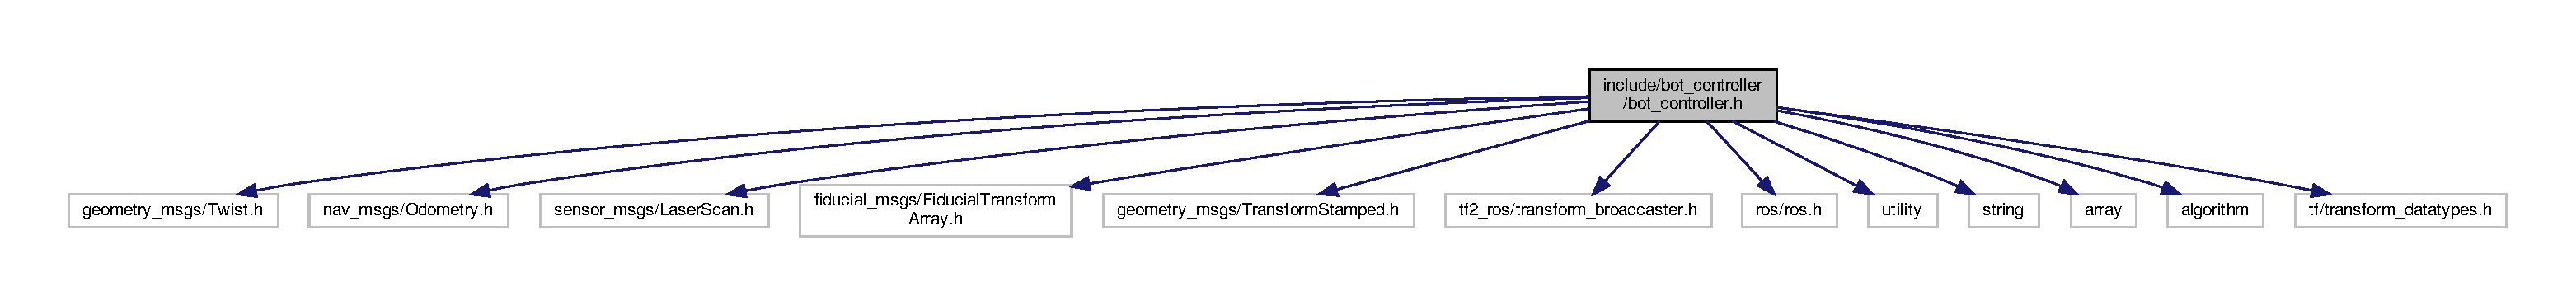
\includegraphics[width=350pt]{bot__controller_8h__incl}
\end{center}
\end{figure}
This graph shows which files directly or indirectly include this file\+:\nopagebreak
\begin{figure}[H]
\begin{center}
\leavevmode
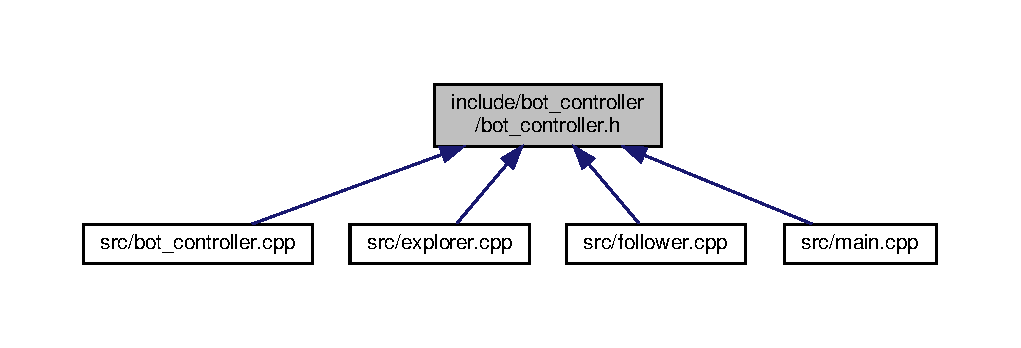
\includegraphics[width=300pt]{bot__controller_8h__dep__incl}
\end{center}
\end{figure}
\subsection*{Classes}
\begin{DoxyCompactItemize}
\item 
class \hyperlink{class_bot___controller}{Bot\+\_\+\+Controller}
\begin{DoxyCompactList}\small\item\em Controller class to drive a turtlebot. \end{DoxyCompactList}\end{DoxyCompactItemize}

\hypertarget{explorer_8h}{}\section{include/explorer/explorer.h File Reference}
\label{explorer_8h}\index{include/explorer/explorer.\+h@{include/explorer/explorer.\+h}}
{\ttfamily \#include $<$geometry\+\_\+msgs/\+Twist.\+h$>$}\newline
{\ttfamily \#include $<$geometry\+\_\+msgs/\+Quaternion.\+h$>$}\newline
{\ttfamily \#include $<$geometry\+\_\+msgs/\+Transform\+Stamped.\+h$>$}\newline
{\ttfamily \#include $<$nav\+\_\+msgs/\+Odometry.\+h$>$}\newline
{\ttfamily \#include $<$sensor\+\_\+msgs/\+Laser\+Scan.\+h$>$}\newline
{\ttfamily \#include $<$fiducial\+\_\+msgs/\+Fiducial\+Transform\+Array.\+h$>$}\newline
{\ttfamily \#include $<$move\+\_\+base\+\_\+msgs/\+Move\+Base\+Action.\+h$>$}\newline
{\ttfamily \#include $<$tf2\+\_\+ros/transform\+\_\+broadcaster.\+h$>$}\newline
{\ttfamily \#include $<$tf2\+\_\+ros/transform\+\_\+listener.\+h$>$}\newline
{\ttfamily \#include $<$tf2/\+Linear\+Math/\+Quaternion.\+h$>$}\newline
{\ttfamily \#include $<$actionlib/client/simple\+\_\+action\+\_\+client.\+h$>$}\newline
{\ttfamily \#include $<$ros/ros.\+h$>$}\newline
{\ttfamily \#include $<$utility$>$}\newline
{\ttfamily \#include $<$string$>$}\newline
{\ttfamily \#include $<$array$>$}\newline
{\ttfamily \#include $<$algorithm$>$}\newline
{\ttfamily \#include $<$iostream$>$}\newline
{\ttfamily \#include $<$tf/transform\+\_\+datatypes.\+h$>$}\newline
{\ttfamily \#include $<$cmath$>$}\newline
Include dependency graph for explorer.\+h\+:\nopagebreak
\begin{figure}[H]
\begin{center}
\leavevmode
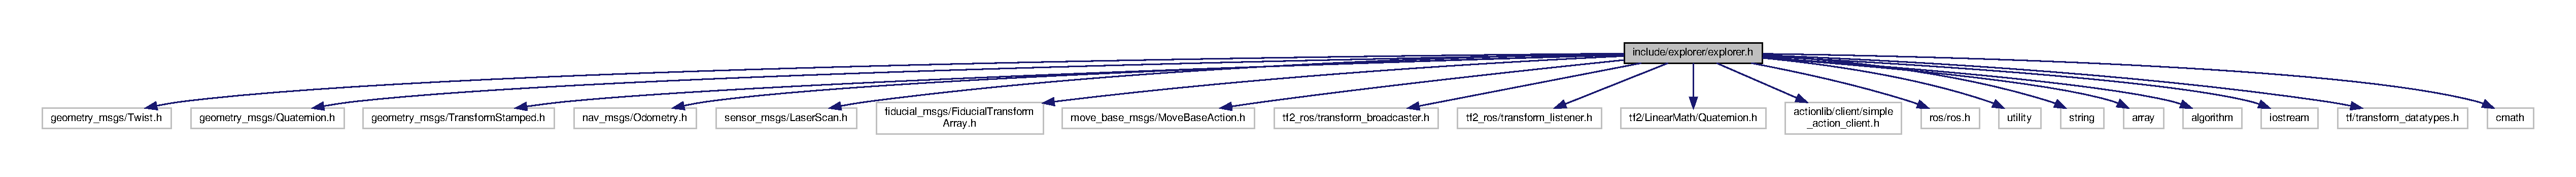
\includegraphics[width=350pt]{explorer_8h__incl}
\end{center}
\end{figure}
This graph shows which files directly or indirectly include this file\+:\nopagebreak
\begin{figure}[H]
\begin{center}
\leavevmode
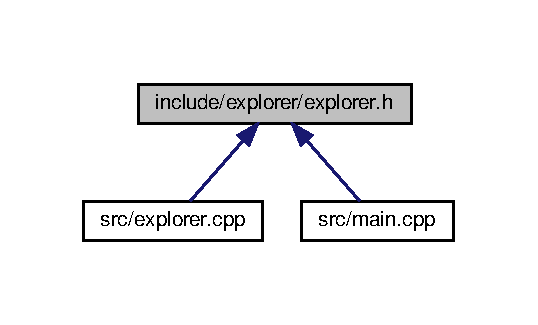
\includegraphics[width=258pt]{explorer_8h__dep__incl}
\end{center}
\end{figure}
\subsection*{Classes}
\begin{DoxyCompactItemize}
\item 
class \hyperlink{class_explorer}{Explorer}
\begin{DoxyCompactList}\small\item\em A class that inherits from Bot\+\_\+contreoller to control the explorer and exploration algorithm. \end{DoxyCompactList}\end{DoxyCompactItemize}

\hypertarget{follower_8h}{}\section{include/follower/follower.h File Reference}
\label{follower_8h}\index{include/follower/follower.\+h@{include/follower/follower.\+h}}
{\ttfamily \#include \char`\"{}../include/bot\+\_\+controller/bot\+\_\+controller.\+h\char`\"{}}\newline
Include dependency graph for follower.\+h\+:
\nopagebreak
\begin{figure}[H]
\begin{center}
\leavevmode
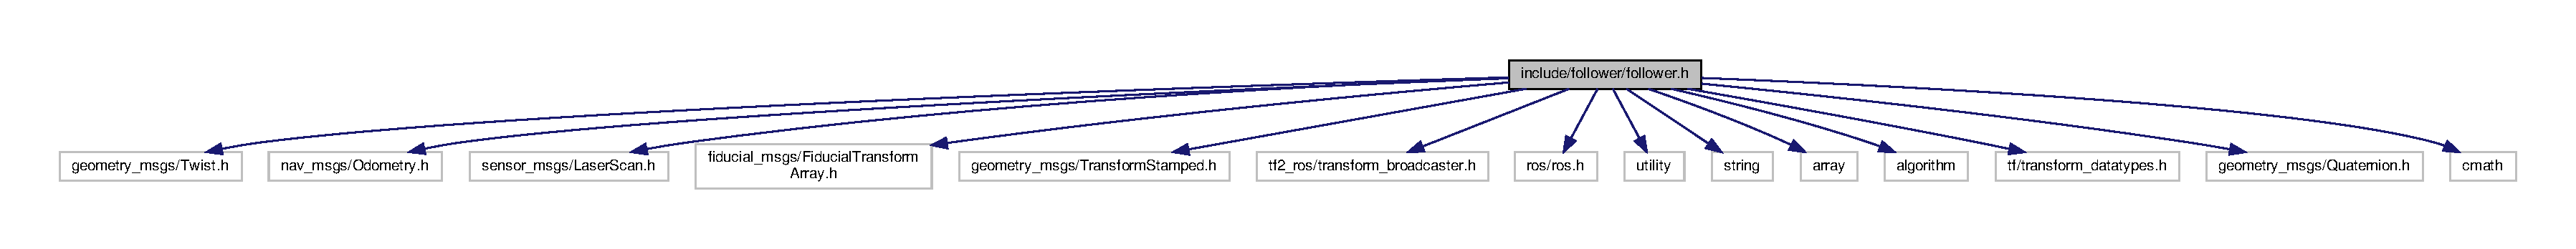
\includegraphics[width=209pt]{follower_8h__incl}
\end{center}
\end{figure}
This graph shows which files directly or indirectly include this file\+:
\nopagebreak
\begin{figure}[H]
\begin{center}
\leavevmode
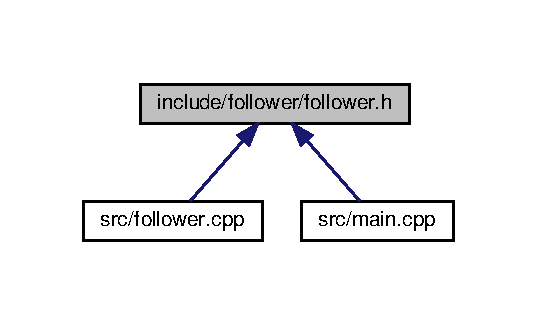
\includegraphics[width=258pt]{follower_8h__dep__incl}
\end{center}
\end{figure}
\subsection*{Classes}
\begin{DoxyCompactItemize}
\item 
class \hyperlink{class_follower}{Follower}
\begin{DoxyCompactList}\small\item\em Public Inheritance Child class of Bot\+\_\+controller Class to go to Ar\+Uco markers found by \hyperlink{class_explorer}{Explorer} child. \end{DoxyCompactList}\end{DoxyCompactItemize}

\hypertarget{_r_e_a_d_m_e_8md}{}\section{R\+E\+A\+D\+M\+E.\+md File Reference}
\label{_r_e_a_d_m_e_8md}\index{R\+E\+A\+D\+M\+E.\+md@{R\+E\+A\+D\+M\+E.\+md}}

\hypertarget{bot__controller_8cpp}{}\section{src/bot\+\_\+controller.cpp File Reference}
\label{bot__controller_8cpp}\index{src/bot\+\_\+controller.\+cpp@{src/bot\+\_\+controller.\+cpp}}
{\ttfamily \#include \char`\"{}bot\+\_\+controller.\+h\char`\"{}}\newline
{\ttfamily \#include $<$geometry\+\_\+msgs/\+Quaternion.\+h$>$}\newline
{\ttfamily \#include $<$tf/transform\+\_\+datatypes.\+h$>$}\newline
{\ttfamily \#include $<$cmath$>$}\newline
Include dependency graph for bot\+\_\+controller.\+cpp\+:\nopagebreak
\begin{figure}[H]
\begin{center}
\leavevmode
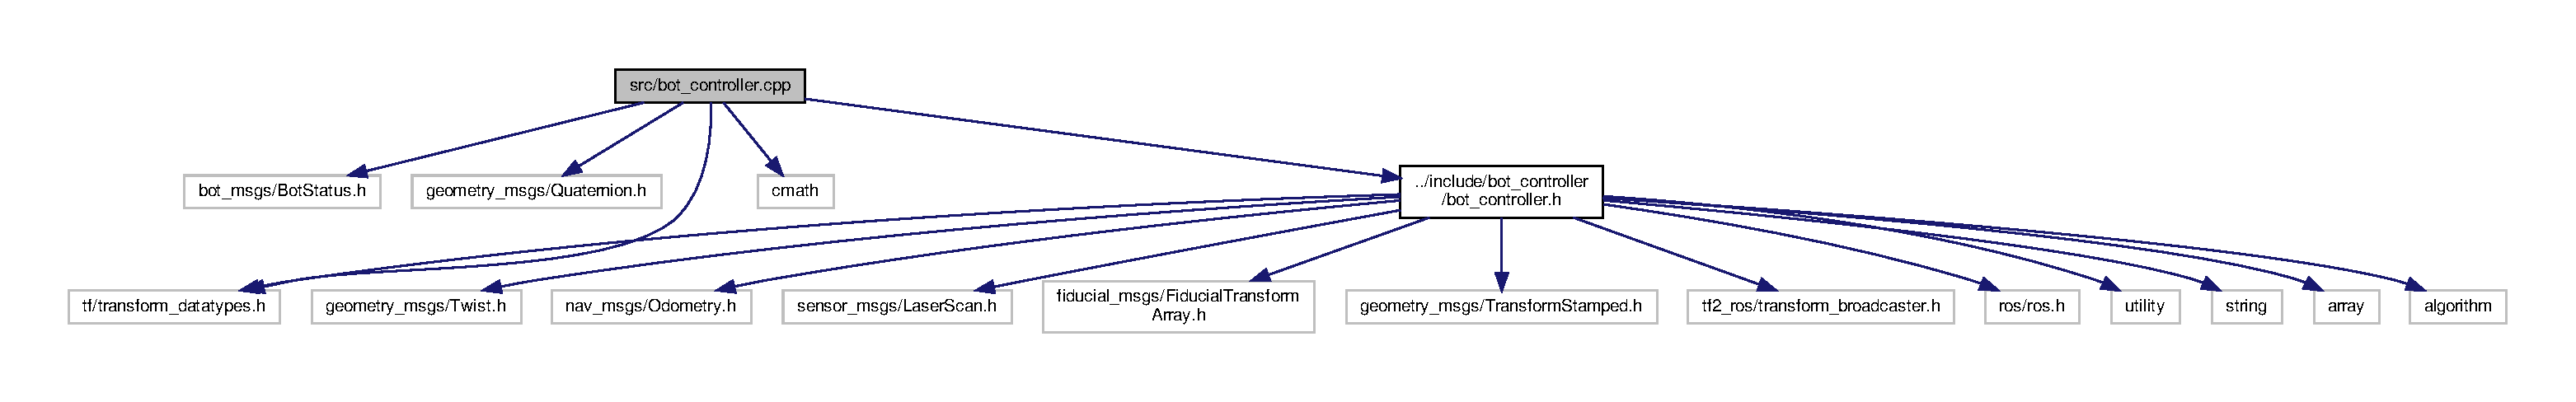
\includegraphics[width=350pt]{bot__controller_8cpp__incl}
\end{center}
\end{figure}

\hypertarget{explorer_8cpp}{}\section{src/explorer.cpp File Reference}
\label{explorer_8cpp}\index{src/explorer.\+cpp@{src/explorer.\+cpp}}


\hyperlink{class_aruco_node}{Aruco\+Node}.  


{\ttfamily \#include \char`\"{}../include/explorer/explorer.\+h\char`\"{}}\newline
Include dependency graph for explorer.\+cpp\+:
\nopagebreak
\begin{figure}[H]
\begin{center}
\leavevmode
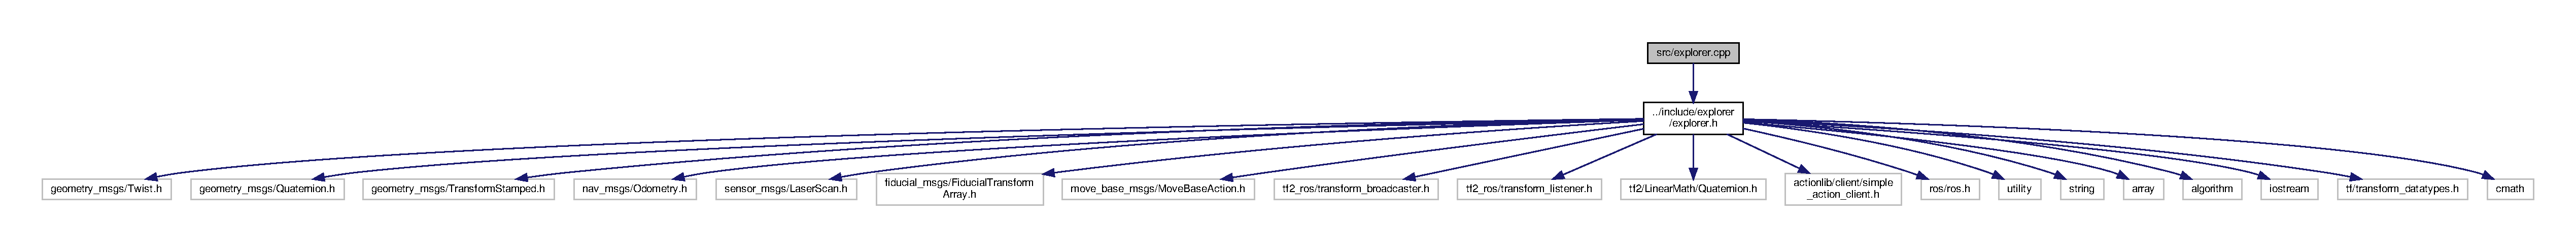
\includegraphics[width=350pt]{explorer_8cpp__incl}
\end{center}
\end{figure}
\subsection*{Functions}
\begin{DoxyCompactItemize}
\item 
std\+::array$<$ std\+::array$<$ double, 2 $>$, 4 $>$ \hyperlink{explorer_8cpp_a61450d29adf96573b7eec19cb2fa8156}{get\+\_\+goals} ()
\begin{DoxyCompactList}\small\item\em Get the goals object from aruco\+\_\+lookup.\+yaml. \end{DoxyCompactList}\end{DoxyCompactItemize}


\subsection{Detailed Description}
\hyperlink{class_aruco_node}{Aruco\+Node}. 

\hyperlink{class_explorer}{Explorer} Robot.

\begin{DoxyAuthor}{Author}
809Y Final Project Group 5 
\end{DoxyAuthor}
\begin{DoxyVersion}{Version}
0.\+1 
\end{DoxyVersion}
\begin{DoxyDate}{Date}
2021-\/12-\/12
\end{DoxyDate}
\begin{DoxyCopyright}{Copyright}
Copyright (c) 2021 
\end{DoxyCopyright}


\subsection{Function Documentation}
\mbox{\Hypertarget{explorer_8cpp_a61450d29adf96573b7eec19cb2fa8156}\label{explorer_8cpp_a61450d29adf96573b7eec19cb2fa8156}} 
\index{explorer.\+cpp@{explorer.\+cpp}!get\+\_\+goals@{get\+\_\+goals}}
\index{get\+\_\+goals@{get\+\_\+goals}!explorer.\+cpp@{explorer.\+cpp}}
\subsubsection{\texorpdfstring{get\+\_\+goals()}{get\_goals()}}
{\footnotesize\ttfamily std\+::array$<$std\+::array$<$double,2$>$,4$>$ get\+\_\+goals (\begin{DoxyParamCaption}{ }\end{DoxyParamCaption})}



Get the goals object from aruco\+\_\+lookup.\+yaml. 

\begin{DoxyReturn}{Returns}
std\+::array$<$std\+::array$<$double,2$>$,4$>$ 
\end{DoxyReturn}


Definition at line 82 of file explorer.\+cpp.


\hypertarget{follower_8cpp}{}\section{src/follower.cpp File Reference}
\label{follower_8cpp}\index{src/follower.\+cpp@{src/follower.\+cpp}}


\hyperlink{class_follower}{Follower} Robot.  


{\ttfamily \#include \char`\"{}../include/bot\+\_\+controller/bot\+\_\+controller.\+h\char`\"{}}\newline
{\ttfamily \#include \char`\"{}../include/follower/follower.\+h\char`\"{}}\newline
Include dependency graph for follower.\+cpp\+:
\nopagebreak
\begin{figure}[H]
\begin{center}
\leavevmode
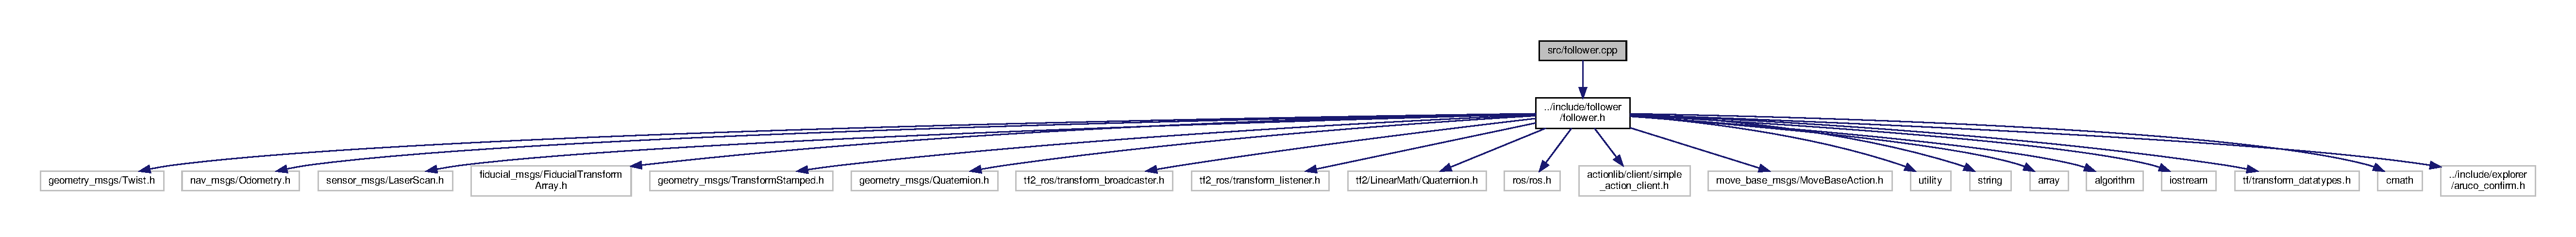
\includegraphics[width=350pt]{follower_8cpp__incl}
\end{center}
\end{figure}


\subsection{Detailed Description}
\hyperlink{class_follower}{Follower} Robot. 

\begin{DoxyAuthor}{Author}
809Y Final Project Group 5 
\end{DoxyAuthor}
\begin{DoxyVersion}{Version}
0.\+1 
\end{DoxyVersion}
\begin{DoxyDate}{Date}
2021-\/12-\/12
\end{DoxyDate}
\begin{DoxyCopyright}{Copyright}
Copyright (c) 2021 
\end{DoxyCopyright}

\hypertarget{main_8cpp}{}\section{src/main.cpp File Reference}
\label{main_8cpp}\index{src/main.\+cpp@{src/main.\+cpp}}


E\+N\+P\+M809Y Final Project Group 5.  


{\ttfamily \#include $<$actionlib/client/simple\+\_\+action\+\_\+client.\+h$>$}\newline
{\ttfamily \#include $<$fiducial\+\_\+msgs/\+Fiducial\+Transform\+Array.\+h$>$}\newline
{\ttfamily \#include $<$geometry\+\_\+msgs/\+Twist.\+h$>$}\newline
{\ttfamily \#include $<$move\+\_\+base\+\_\+msgs/\+Move\+Base\+Action.\+h$>$}\newline
{\ttfamily \#include $<$tf2/\+Linear\+Math/\+Quaternion.\+h$>$}\newline
{\ttfamily \#include $<$tf2\+\_\+ros/transform\+\_\+broadcaster.\+h$>$}\newline
{\ttfamily \#include $<$tf2\+\_\+ros/transform\+\_\+listener.\+h$>$}\newline
{\ttfamily \#include $<$ros/ros.\+h$>$}\newline
{\ttfamily \#include $<$array$>$}\newline
{\ttfamily \#include $<$iostream$>$}\newline
{\ttfamily \#include $<$algorithm$>$}\newline
{\ttfamily \#include $<$utility$>$}\newline
{\ttfamily \#include \char`\"{}../include/follower/follower.\+h\char`\"{}}\newline
{\ttfamily \#include \char`\"{}../include/explorer/explorer.\+h\char`\"{}}\newline
Include dependency graph for main.\+cpp\+:
\nopagebreak
\begin{figure}[H]
\begin{center}
\leavevmode
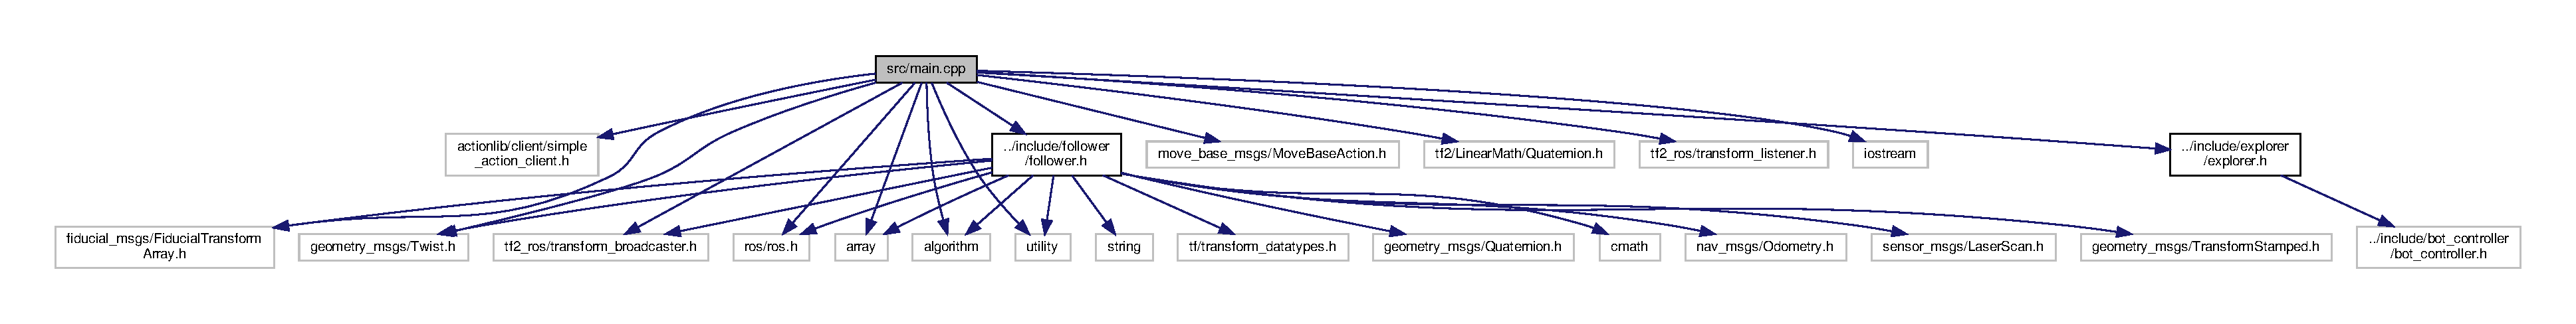
\includegraphics[width=350pt]{main_8cpp__incl}
\end{center}
\end{figure}
\subsection*{Typedefs}
\begin{DoxyCompactItemize}
\item 
typedef actionlib\+::\+Simple\+Action\+Client$<$ move\+\_\+base\+\_\+msgs\+::\+Move\+Base\+Action $>$ \hyperlink{main_8cpp_a21e20cc0b6656ae897b3cbb969b93241}{Move\+Base\+Client}
\end{DoxyCompactItemize}
\subsection*{Functions}
\begin{DoxyCompactItemize}
\item 
void \hyperlink{main_8cpp_a9c2747abcaef4c03d19858e45f59de80}{print\+\_\+usage} (std\+::string error=\char`\"{}\char`\"{})
\item 
void \hyperlink{main_8cpp_a299d89c50484c4d3a597f6b43b65e21c}{broadcast} ()
\item 
void \hyperlink{main_8cpp_aa2baabcf8bc6fb2727c0aade0c1b8efe}{listen} (tf2\+\_\+ros\+::\+Buffer \&tf\+Buffer)
\item 
int \hyperlink{main_8cpp_a3c04138a5bfe5d72780bb7e82a18e627}{main} (int argc, char $\ast$$\ast$argv)
\end{DoxyCompactItemize}


\subsection{Detailed Description}
E\+N\+P\+M809Y Final Project Group 5. 

\begin{DoxyAuthor}{Author}
Jerry Pittman, Jr., Nicholas Novak, Orlandis Smith (\href{mailto:jpittma1@umd.edu}{\tt jpittma1@umd.\+edu}, \href{mailto:nnovak@umd.edu}{\tt nnovak@umd.\+edu}, \href{mailto:osmith15@umd.edu}{\tt osmith15@umd.\+edu}) 
\end{DoxyAuthor}
\begin{DoxyVersion}{Version}
0.\+1 
\end{DoxyVersion}
\begin{DoxyDate}{Date}
2021-\/12-\/11
\end{DoxyDate}
\begin{DoxyCopyright}{Copyright}
Copyright (c) 2021 
\end{DoxyCopyright}


\subsection{Typedef Documentation}
\mbox{\Hypertarget{main_8cpp_a21e20cc0b6656ae897b3cbb969b93241}\label{main_8cpp_a21e20cc0b6656ae897b3cbb969b93241}} 
\index{main.\+cpp@{main.\+cpp}!Move\+Base\+Client@{Move\+Base\+Client}}
\index{Move\+Base\+Client@{Move\+Base\+Client}!main.\+cpp@{main.\+cpp}}
\subsubsection{\texorpdfstring{Move\+Base\+Client}{MoveBaseClient}}
{\footnotesize\ttfamily typedef actionlib\+::\+Simple\+Action\+Client$<$move\+\_\+base\+\_\+msgs\+::\+Move\+Base\+Action$>$ \hyperlink{main_8cpp_a21e20cc0b6656ae897b3cbb969b93241}{Move\+Base\+Client}}



Definition at line 29 of file main.\+cpp.



\subsection{Function Documentation}
\mbox{\Hypertarget{main_8cpp_a299d89c50484c4d3a597f6b43b65e21c}\label{main_8cpp_a299d89c50484c4d3a597f6b43b65e21c}} 
\index{main.\+cpp@{main.\+cpp}!broadcast@{broadcast}}
\index{broadcast@{broadcast}!main.\+cpp@{main.\+cpp}}
\subsubsection{\texorpdfstring{broadcast()}{broadcast()}}
{\footnotesize\ttfamily void broadcast (\begin{DoxyParamCaption}{ }\end{DoxyParamCaption})}



Definition at line 41 of file main.\+cpp.

\mbox{\Hypertarget{main_8cpp_aa2baabcf8bc6fb2727c0aade0c1b8efe}\label{main_8cpp_aa2baabcf8bc6fb2727c0aade0c1b8efe}} 
\index{main.\+cpp@{main.\+cpp}!listen@{listen}}
\index{listen@{listen}!main.\+cpp@{main.\+cpp}}
\subsubsection{\texorpdfstring{listen()}{listen()}}
{\footnotesize\ttfamily void listen (\begin{DoxyParamCaption}\item[{tf2\+\_\+ros\+::\+Buffer \&}]{tf\+Buffer }\end{DoxyParamCaption})}



Definition at line 62 of file main.\+cpp.

\mbox{\Hypertarget{main_8cpp_a3c04138a5bfe5d72780bb7e82a18e627}\label{main_8cpp_a3c04138a5bfe5d72780bb7e82a18e627}} 
\index{main.\+cpp@{main.\+cpp}!main@{main}}
\index{main@{main}!main.\+cpp@{main.\+cpp}}
\subsubsection{\texorpdfstring{main()}{main()}}
{\footnotesize\ttfamily int main (\begin{DoxyParamCaption}\item[{int}]{argc,  }\item[{char $\ast$$\ast$}]{argv }\end{DoxyParamCaption})}



Definition at line 84 of file main.\+cpp.

\mbox{\Hypertarget{main_8cpp_a9c2747abcaef4c03d19858e45f59de80}\label{main_8cpp_a9c2747abcaef4c03d19858e45f59de80}} 
\index{main.\+cpp@{main.\+cpp}!print\+\_\+usage@{print\+\_\+usage}}
\index{print\+\_\+usage@{print\+\_\+usage}!main.\+cpp@{main.\+cpp}}
\subsubsection{\texorpdfstring{print\+\_\+usage()}{print\_usage()}}
{\footnotesize\ttfamily void print\+\_\+usage (\begin{DoxyParamCaption}\item[{std\+::string}]{error = {\ttfamily \char`\"{}\char`\"{}} }\end{DoxyParamCaption})}



Definition at line 34 of file main.\+cpp.


%--- End generated contents ---

% Index
\backmatter
\newpage
\phantomsection
\clearemptydoublepage
\addcontentsline{toc}{chapter}{Index}
\printindex

\end{document}
